\documentclass{article}
\usepackage[rightcaption]{sidecap}
\usepackage{graphicx} % Required for inserting images
\usepackage{multirow}
\usepackage[top=4cm, bottom=4cm, left=3cm, right=3cm]{geometry}
\usepackage[labelfont=bf, justification=raggedright, singlelinecheck=false]{caption}
\usepackage[european, americanvoltages]{circuitikz} % Per i circuiti
\usepackage{pgfplots}
\pgfplotsset{compat=1.18} % Ottimizza la compatibilità di PGFPlots
\usepgfplotslibrary{groupplots} % Consente di allineare modulo e fase
\newcommand\tab[1][1cm]{\hspace*{#1}}
\usepackage[T1]{fontenc}
\usepackage{appendix}
\usepackage{tabularx}
\usepackage{float}
\usepackage{tcolorbox}
\usepackage{amsmath}
\usepackage{amssymb}
\usepackage{eso-pic} % for \BgThispage
\usepackage{tikz}
\usepackage{titlesec}
\usepackage{tocloft}
\usetikzlibrary{arrows.meta}
\usepackage[pages=some]{background}
\usepackage[italian]{babel}
\usepackage[colorlinks=true, linkcolor=black, citecolor=black, filecolor=black, urlcolor=blue]{hyperref}
\addto\captionsitalian{\renewcommand{\contentsname}{Indice}}
\backgroundsetup{scale=1.5,anchor=right,angle=0,opacity=0.1,contents={
\includegraphics[scale=1]{Misc/logo_standard (1).png}}}

% FORMATTAZIONE SOTTOTITOLI
%-----------------------------------------------------------
\titleformat{\subsection}
{\normalfont\Large\bfseries}{\thesubsection}{1em}{}

\titleformat{\section}
{\normalfont\Large\bfseries}{\thesection}{1em}{}
%-----------------------------------------------------------

% FORMATTAZIONE INDICE
%-----------------------------------------------------------
\renewcommand{\cftsecfont}{\normalfont\Large\bfseries}
\renewcommand{\cftsecpagefont}{\normalfont\Large\bfseries}

\renewcommand{\cftsubsecfont}{\normalfont\Large}
\renewcommand{\cftsubsecpagefont}{\normalfont\Large}

\setlength{\cftbeforesecskip}{0.5cm} 
\setlength{\cftbeforesubsecskip}{0.3cm}
%-----------------------------------------------------------

% TITOLO
%-----------------------------------------------------------
\title{
    Relazione : Amplificatori Operazionali e Filtri RC \\ 
    \vspace{0.3cm} 
    \Large Gruppo 100
}
%-----------------------------------------------------------

% AUTORI
%-----------------------------------------------------------
\author{
  Lorenzo Allocco \\ -- Mat. 0612709084
  \\ \\
  Riccardo La Porta \\ -- Mat. 0612709691
  \\ \\
  Francesco Grimaldi \\ -- Mat. 0612708839
  \\ \\
  Alessandro Altieri \\ -- Mat. 0612709239
}

\date{13 Giugno 2026}

\begin{document}
\BgThispage

\AddToShipoutPictureBG*{
  \begin{tikzpicture}[remember picture, overlay]
    \node [anchor=north west, inner sep=30pt] at (current page.north west)
      {
\includegraphics[height=1.5cm]{Misc/diem (1).png}};
  \end{tikzpicture}
}
%-----------------------------------------------------------

\maketitle

% INDICE
%-----------------------------------------------------------
\newpage
\tableofcontents
\newpage
%-----------------------------------------------------------

\section{Obiettivi della prova}
  La seguente relazione si pone come obiettivo quello di descrivere l'esperienza di laboratorio tenutasi
  nell'ambito del corso di Tecnologie Elettriche per l'informatica Industriale.\\ \\
  Lo scopo è quello di illustrare nel dettaglio come funzionano le varie tipologie di filtri RC 
  dimensionando opportunamente i vari componenti e progettando la configurazione dei vari blocchi,
  adoperando anche gli amplificatori operazionali. \\ \\
  In particolare, si cerca di evidenziare le proprietà filtranti dei componenti dinamici (come il condensatore)
  e come questi possono essere opportunamente inseriti in un contesto circuitale per manipolare i segnali. \\ \\
  Riassumendo tutto, l'esperienza di laboratorio ha come obiettivo:
  \begin{itemize}
      \item Dimensionare opportunamente i componenti per ricreare dei filtri con delle specifiche frequenze di taglio,
            in particolare: \\
            {-} un filtro passa-basso del primo ordine \\
            {-} un filtro passa-banda
      \item Estrarre le componenti armoniche desiderate da segnali misti
      \item Verificare con il diagramma di Bode se i risultati ottenuti sono coerenti
  \end{itemize}
\newpage

% ==========================================
% SCHEMI
% ==========================================

\section{Schemi}

  % ==========================================
  % FIGURA 1: FILTRO PASSA-BASSO (LOW-PASS)
  % ==========================================
  \begin{figure}[H]
      \centering
      \begin{circuitikz}[scale=1.2] 
          % Generatore di ingresso
          \draw (0,0) to[vsourcesin, l=$V_{in}$] (0,2)
          % Resistore R sulla linea di segnale
          to[R, l=$R_{L}$] (3,2)
          % Condensatore C in parallelo verso massa
          to[short] (4,2)
          to[C, l=$C_{L}$] (4,0);
          
          % Morsetti di uscita Vout
          \draw (4,2) to[short, -o] (5,2) node[above] {$V_{out}$};
          \draw (4,0) to[short, -o] (5,0);
          
          % Chiusura linea inferiore di massa
          \draw (4,0) to[short] (0,0) node[ground] {};
      \end{circuitikz}
      \caption{Schema elettrico del filtro RC passa-basso (Low-Pass L(s)).}
      \label{fig:filtro_passabasso}
  \end{figure}

  % ==========================================
  % FIGURA 2: FILTRO PASSA-ALTO (HIGH-PASS)
  % ==========================================
  \begin{figure}[H]
      \centering
      \begin{circuitikz}[scale=1.2] 
          % Generatore di ingresso
          \draw (0,0) to[vsourcesin, l=$V_{in}$] (0,2)
          % Condensatore C in serie sulla linea di segnale
          to[C, l=$C_{H}$] (3,2)
          % Resistore R in parallelo verso massa
          to[short] (4,2)
          to[R, l=$R_{H}$] (4,0);
          
          % Morsetti di uscita Vout
          \draw (4,2) to[short, -o] (5,2) node[above] {$V_{out}$};
          \draw (4,0) to[short, -o] (5,0);
          
          % Chiusura linea inferiore di massa
          \draw (4,0) to[short] (0,0) node[ground] {};
      \end{circuitikz}
      \caption{Schema elettrico del filtro RC passa-alto (High-Pass H(s)).}
      \label{fig:filtro_passaalto}
  \end{figure}

  % ==========================================
  % FIGURA 3: FILTRO PASSA-BANDA (BAND-PASS)
  % ==========================================
  \begin{figure}[H]
      \centering
      \begin{circuitikz}[scale=0.9, transform shape]
          % === LINEA DI SEGNALE PRINCIPALE DEI FILTRI A QUOTA Y=2 ===
          % === LINEA DI MASSA GENERALE A QUOTA Y=0 ===

          % --- PRIMO STADIO: FILTRO PASSA-BASSO ---
          % Generatore di ingresso
          \draw (0,0) to[vsourcesin, l=$V_{in}$] (0,2)
          % Condensatore C1 a quota Y=2 
          to[R, l=$R_1$] (3.5,2)
          % Resistenza R1 verso massa
          to[C, l=$C_1$] (3.5,0);
          % Filo inferiore di massa per il primo stadio
          \draw (3.5,0) -- (0,0) node[ground] {};

          % --- OPERAZIONALE SPOSTATO IN GIÙ ---
          \draw (7.5,2) node[op amp, anchor=out] (opamp) {}; 
          
          % --- COLLEGAMENTO AL PIN '+' SQUADRATO ---
          \draw (3.5,2) -- (4.5,2) -- (4.5,1.5) -- (opamp.+);
          
          % --- RETROAZIONE A RETTANGOLO CHE CIRCONDA L'OPERAZIONALE ---
          \draw (opamp.out) -- (7.5,3.5) -- (5.12,3.5) -- (opamp.-);

          % --- SECONDO STADIO: FILTRO PASSA-ALTO (LINEA RETTA DALL'USCITA) ---
          % Dal punto di deviazione (7.2,2) andiamo dritti verso C2 senza interruzioni o scalini
          \draw(11,0)
          % Condensatore C2 drittissimo a quota Y=2
          to[R, l=$R_2$] (11,2)
          % Resistenza R2 verso massa
          to[C, l=$C_2$] (opamp.out);
          
          % Morsetti finali di uscita Vout dritti
          \draw (11,2) to[short, -o] (12,2) node[above] {$V_{out}$};
          \draw (11,0) to[short, -o] (12,0);

          % --- LINEA DI MASSA COMUNE ORIZZONTALE ---
          \draw (11,0) -- (3.5,0); 
          
      \end{circuitikz}
      \caption{Schema elettrico del filtro RC passa-banda con Op-Amp in configurazione \\ Voltage Follower (Band-pass B(s)).}
      \label{fig:filtro_passabanda}
  \end{figure}

\newpage

% ==========================================
% ELENCO DEI COMPONENTI
% ==========================================

\section{Elenco dei componenti}
  \subsection{\textit{Filtro Passa-Basso}}
    \begin{itemize}
        \item Condensatore ($C_{L}$): 0.1 $\mu$F
        \item Resistore ($R_{L}$): 10 k$\Omega$
    \end{itemize}

    \subsection{\textit{Filtro Passa-Banda}}
    \begin{itemize}
        \item Condensatore ($C_{1}$): 0.1 $\mu$F
        \item Condensatore ($C_{2}$): 22 $\mu$F
        \item Resistore ($R_{1}$): 165 $\Omega$
        \item Resistore ($R_{2}$): 330 $\Omega$
    \end{itemize}

\section{Strumenti utilizzati}

La strumentazione utilizzata durante l'esperienza è elencata nella tabella seguente:

  \begin{table}[H]
    \centering

    \begin{tabularx}{\textwidth}{|X|X|X|}
      \hline
      \textbf{Strumento} & \textbf{Modello} & \textbf{Caratteristiche} \\ \hline
      Oscilloscopio Digitale & Hantek 6022BL & 2 canali, 20 MHz, 48 MS/s \\ \hline
      Software & DPO & Software per macchine Windows \\ \hline
      Software & OpenHantek & Software open source disponibile su macchine linux \\ \hline
      Microcontrollore & Raspberry Pi 3 & Clock: 1.2 GHz, 4 porte USB \\ \hline
      BreadBoard & 165x55x10 & 830 fori, 69gr \\ \hline
    \end{tabularx}

    \captionsetup{justification=centering, singlelinecheck=false, font=small}
    \caption{Specifiche della strumentazione di laboratorio.}
  \end{table}

\newpage

\section{FILTRO PASSA-BASSO}

\subsection{Descrizione delle misure effettuate}
  In questo esperimento, l’obiettivo è realizzare un filtro passa-basso composto da
  un resistore e un condensatore. Avendo a disposizione diverse tipologie di questi
  componenti, abbiamo scelto quest'ultimi sulla base di alcune osservazioni:
  \begin{itemize}
    \item Analizziamo la configurazione circuitale in \textit{Figura 1} e consideriamo il diagramma a blocchi e il \textit{Diagramma di Bode}
          del sistema schematizzati come:
          % Disegno del blocco
          \begin{figure}[H]
            \centering
            \begin{tikzpicture}[
                % Definiamo lo stile del blocco centrale per non doverlo ripetere
                blocco/.style={
                    draw, 
                    rectangle, 
                    minimum width=2cm, 
                    minimum height=1.5cm, 
                    line width=1.5pt,
                    align=center
                },
                % Stile per le frecce con la punta marcata
                freccia/.style={
                    ->, 
                    >={Stealth[length=3mm]}, 
                    line width=1.5pt
                }
            ]
                
                % 1. Posizioniamo il blocco centrale con la formula matematica
                \node [blocco] (sistema) at (0,0) {\Large $\frac{1}{R_{L}C_{L}s + 1}$};
                
                % 2. Freccia di ingresso (Vin)
                % Partiamo da sinistra rispetto al blocco (-3,0) e andiamo verso il bordo sinistro del blocco
                \draw [freccia] (-2.5,0) -- (sistema.west);
                % Etichetta Vin rossa sopra la freccia
                \node [text=red, font=\bfseries\Large] at (-1.8,0.5) {$V_{in}$};
                
                % 3. Freccia di uscita (Vout)
                % Partiamo dal bordo destro del blocco e andiamo verso destra (+2.5,0)
                \draw [freccia] (sistema.east) -- (2.5,0);
                % Etichetta Vout rossa sopra la freccia
                \node [text=red, font=\bfseries\Large] at (1.8,0.5) {$V_{out}$};
                
            \end{tikzpicture}
            \captionsetup{justification=centering, singlelinecheck=false, font=small}
            \caption{Rappresentazione a blocchi della funzione di trasferimento del filtro \textit{Passa-Basso}.}
            \label{fig:blocco_rc}
          \end{figure}
          
          % Diagramma di Bode
          \begin{figure}[H]
            \centering
            \begin{tikzpicture}
                \begin{axis}[
                    width=11cm, height=6.5cm,   % Leggermente più alto visto che è singolo
                    xmode=log,                  % Asse X logaritmico
                    xmin=1, xmax=10000,         % Range frequenze da 1 Hz a 10 kHz
                    xlabel={Frequenza [Hz]},
                    ylabel={Magnitudo [dB]},
                    ymin=-40, ymax=5,
                    ytick={-30, -20, -10, -3, 0}, % Tick a -3 dB per la frequenza di taglio
                    grid=both,
                    minor grid style={dashed, gray!30},
                    major grid style={gray!60},
                    tick label style={font=\footnotesize},
                    label style={font=\small}
                ]
                
                % Funzione analitica del solo filtro passa-basso: 1 / sqrt(1 + (2*pi*x*tau)^2)
                \addplot[red, thick, domain=1:10000, samples=200] 
                    {20*log10( 1 / sqrt(1 + (2*pi*x*0.001)^2) )};
                    
                \end{axis}
            \end{tikzpicture}
            
            % PROPRIETÀ INLINE: Applica la formattazione solo a questa caption
            \captionsetup{justification=centering, singlelinecheck=false, font=small}
            \caption{Diagramma di Bode (Modulo) del filtro passa-basso}
            \label{fig:bode_passabasso_modulo}
          \end{figure}

          Possiamo notare come questo sistema così configurato agisca come previsto,
          visto che reagisce alle basse frequenze (fino ad arrivare alla \textit{Frequenza di Taglio})
          con un guadagno unitario, mentre reagisce alle alte frequenze con un guadagno sempre più
          piccolo all'aumentare della frequenza con una variazione di -20 dB/dec. 
    \newpage

    \item Dalla teoria dei sistemi, è facile convincersi che per migliorare le prestazioni di
          filtri di questo tipo bisogna aumentare la velocità con cui il guadagno si abbassa per
          le frequenze oltre quella di taglio ($f_{T}$). Inoltre è facile ricavare una formula per
          calcolare $f_{T}$ visto che guardando la funzione di trasferimento osserviamo che la 
          \textit{pulsazione di rottura} ($\omega_{r}$) vale esattamente
          \boldmath{$\omega_{r}$ = $\frac{1}{R_{L}C_{L}}$}, quindi di conseguenza: \\
          \begin{equation}
            \boxed{f_{T} = \frac{1}{2\pi R_{L}C_{L}}}
          \end{equation}

    \item Per arrivare a scegliere accuratamente la resistenza e il condensatore adatti al circuito
          dobbiamo anche osservare che, data la configurazione del circuito in \textit{Figura 1}, la scelta
          del dimensionamento della resistenza può incidere sulla riuscita finale dell'esperimento visto che
          scegliendo un valore troppo basso quest'ultima tenderà al comportamento di un cortocircuito
          mentre scegliendo un valore troppo alto quest'ultima tenderà al comportamento di un'aperto. Il
          valore scelto in fase di progettazione è stato $R_{L}$ = 10k$\Omega$ essendo un giusto compromesso tra
          i due casi descritti in precedenza, evitando così di ridurre significativamente la sensibilità del
          circuito o magari, in alcuni casi, di danneggiarlo.

    \item Ora sulla base del dimensionamento effettuato al punto precedente, possiamo scegliere il valore della
          capacità del condensatore usando la formula ricavata dall'analisi del diagramma di Bode. La capacità
          selezionata in fase progettuale tra i componenti a disposizione è stata $C_{L}$ = 0.1$\mu$F. 

    \item Successivamente abbiamo proceduto alla misurazione effettiva dei paramentri reali dei componenti
          riscontrando il corretto funzionamento di questi, visto il discostamento irrilevante dei valori misurati
          da quelli nominali. Si è scelto quindi di trascurare le differenze tra i valori nominali e quelli misurati
          procedendo così a calcolare la $f_{T}$ come:
          \begin{equation}
            \boxed{f_{T} = \frac{1}{2\pi R_{L}C_{L}} = \frac{1}{2\pi \cdot 10^4 \cdot 10^{-7}} \approx 159.15 \text{ Hz} \approx 160 \text{ Hz}}
          \end{equation}
  \end{itemize}
\newpage

\subsection{Risultati}
    \begin{itemize}
      \item Arrivati a queste conclusioni, possiamo illustrare i risultati ottenuti con le misurazioni all'oscilloscopio:
            \begin{figure}[H]
              \centering
              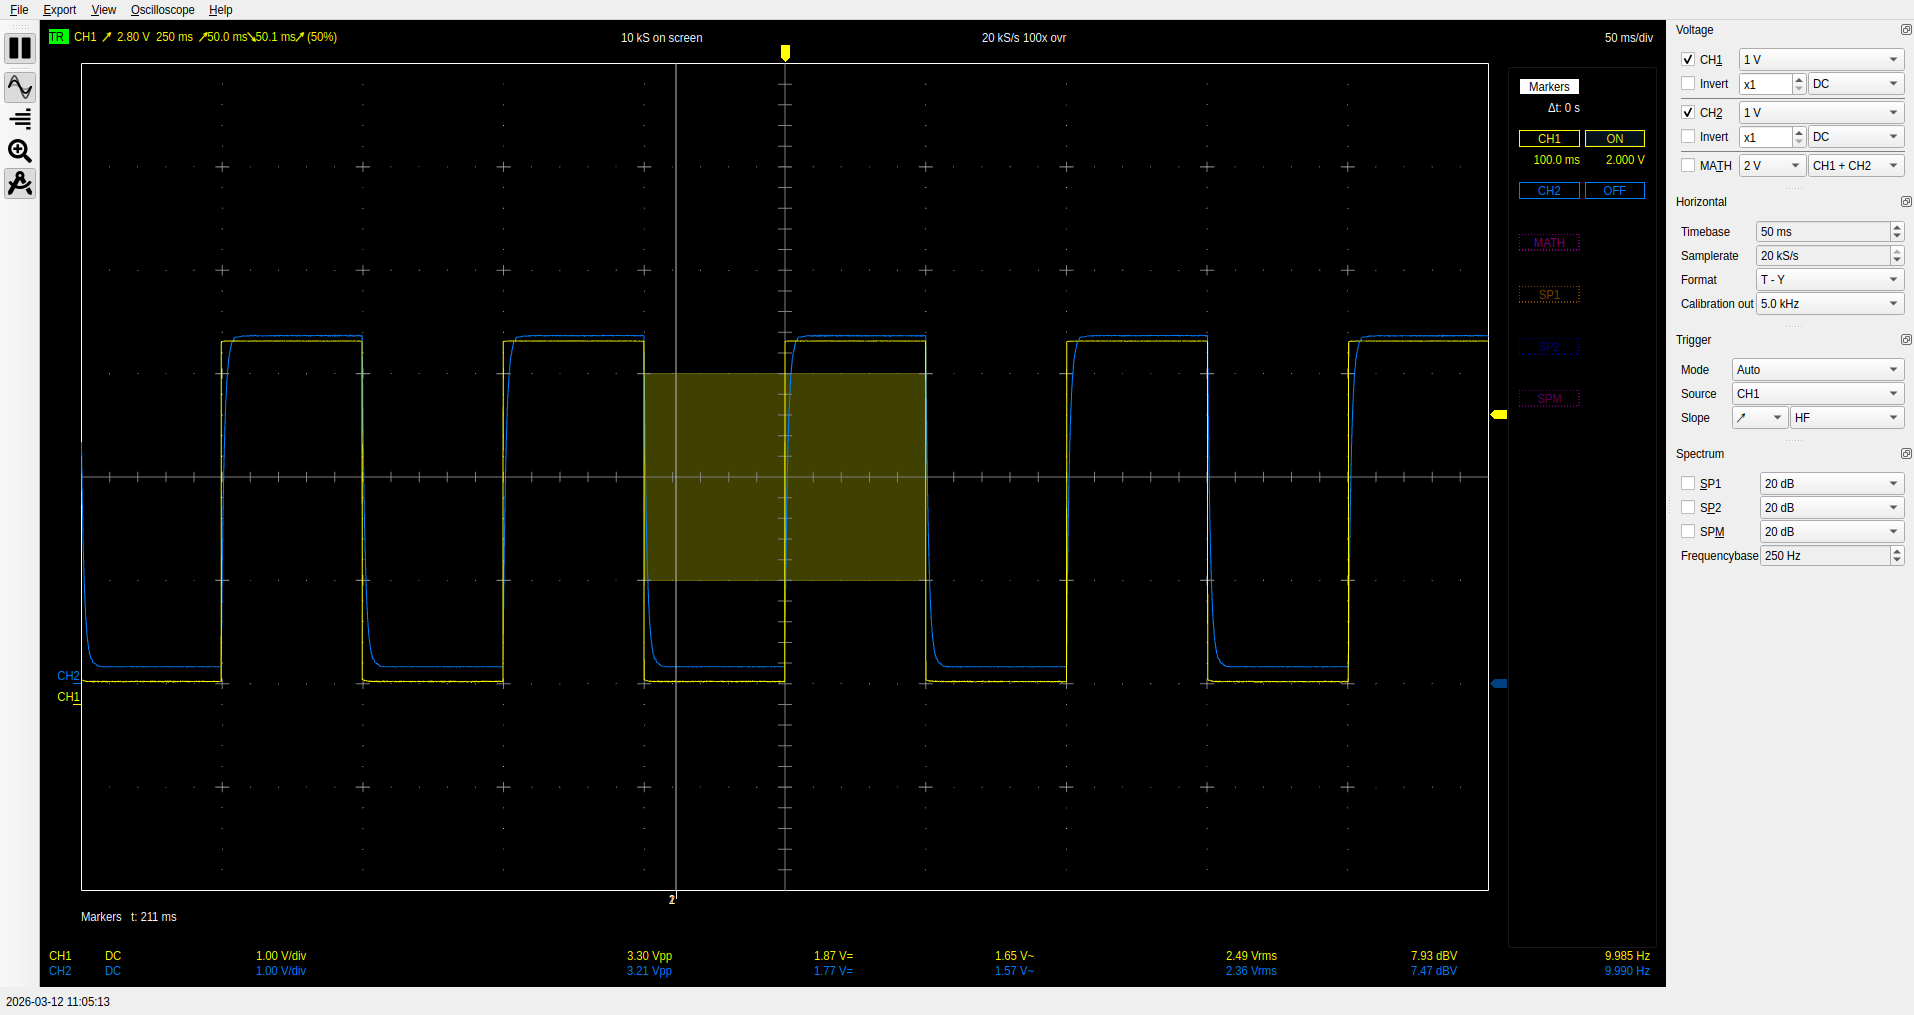
\includegraphics[width=0.7\textwidth]{Misc/10hz LPF.png}
              \captionsetup{justification=centering, singlelinecheck=false, font=small}
              \caption{Onda quadra a 10 Hz}
            \end{figure}

            \begin{figure}[H]
              \centering
              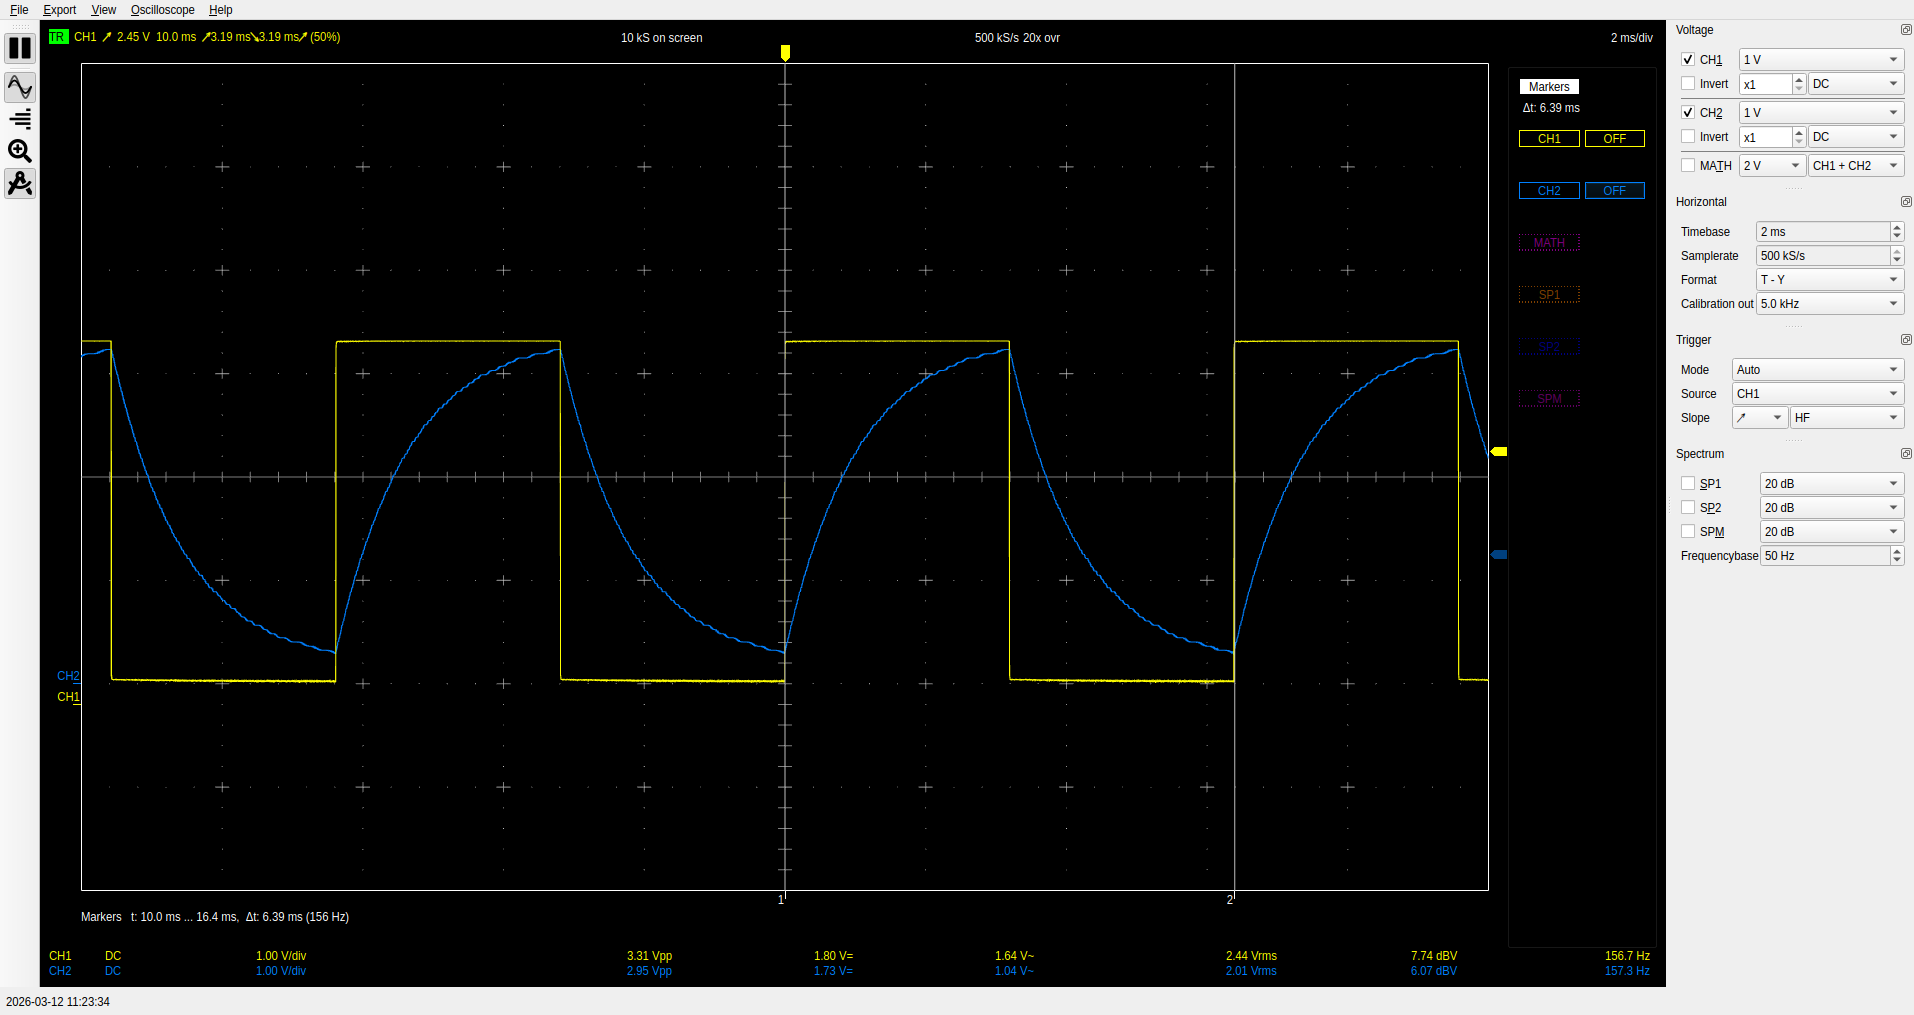
\includegraphics[width=0.7\textwidth]{Misc/160hz LPF.png}
              \captionsetup{justification=centering, singlelinecheck=false, font=small}
              \caption{Onda quadra a 160 Hz}
            \end{figure}

            \begin{figure}[H]
              \centering
              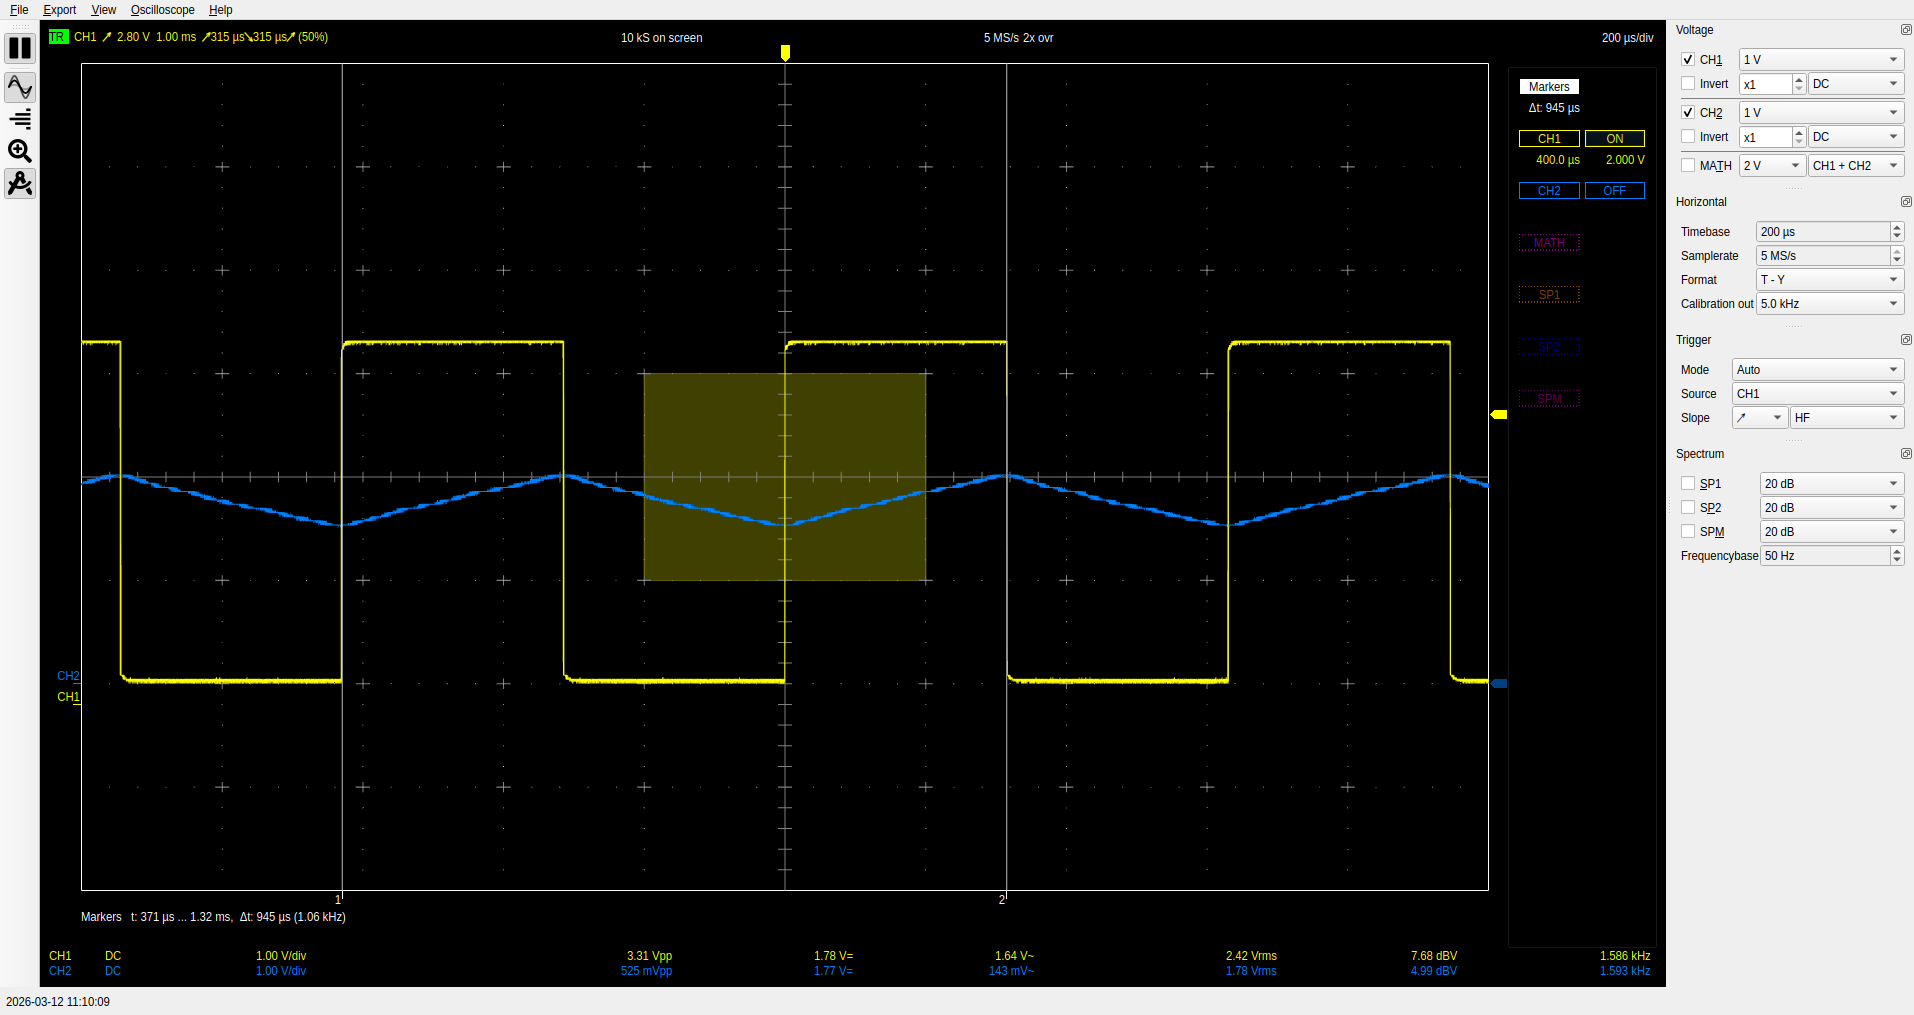
\includegraphics[width=0.7\textwidth]{Misc/2khz LPF.png}
              \captionsetup{justification=centering, singlelinecheck=false, font=small}
              \caption{Onda quadra a 2 kHz}
            \end{figure}

      \item Possiamo subito notare come nel primo caso in \textit{Figura 6} abbiamo in uscita un segnale abbastanza simile 
            all’onda quadra a 10 Hz in ingresso al sistema. E’ ragionevole pensare che sia così visto che la frequenza di 
            questo segnale è dell'ordine di una decade inferiore ad $f_{T}$. Infatti è facile dimostrare, guardando il diagramma 
            di Bode, che il segnale in uscita avrebbe dovuto essere ampio il 99,8\% del segnale originale, perfettamente in accordo
            con i risultati in figura e il calcolo del modulo come segue:
            \begin{equation}
              \boxed{|L(f)| = |L(10)| = \frac{1}{\sqrt{1 + \left(\frac{10}{159.15}\right)^2}} \approx 99,8\%}
            \end{equation}

            Il valore picco-picco in figura è di 3,21V a fronte dei 3,3V del segnale in ingresso. Abbiamo ottenuto un'ampiezza del 97,2\%
            del segnale originale, perfettamente in accordo con i risultati teorici attesi.

      \item Nel secondo caso, in \textit{Figura 7}, con un onda quadra a 160 Hz, notiamo un taglio molto più evidente visto che
            ci troviamo in prossimità di $f_{T}$. L’uscita inizia ad assomigliare di più ad una sinusoide che, in condizioni ideali,
            è proprio ciò che dovremmo aspettarci. Essendo che si tratta di un filtro del primo ordine, il taglio in corrispondenza
            di $f_{T}$ è molto dolce. Basta pensare che addirittura una decade dopo $f_{T}$ (1600 Hz), il diagramma di Bode segna
            un'attenuazione prevista di un fattore 10 (ancora troppo per essere considerato trascurabile). Il segnale in questione
            è un onda quadra a 160 Hz, composta quindi da un contenuto armonico abbastanza rilevante (tutte le armoniche multiple dispari di
            160 Hz, tipo: 480 Hz, 800 Hz, 1120 Hz, 1440 Hz, etc...), di conseguenza è ragionevole pensare che il risultato ottenuto debba
            essere una sinusoide con i cosiddetti 'angoli vivi' smussati (gli angoli vivi sono frutto delle componenti ad alta frequenza, 
            che in questo caso sono presenti con un ampiezza trascurabile).

      \item Nel terzo caso, con un onda quadra a 2 kHz, abbiamo in uscita qualcosa che assomiglia molto ad una sinusoide molto attenuata,
            più simile ad un onda triangolare (cosiddetta 'a dente di sega'). In condizioni ideali avremmo dovuto assistere ad un segnale costante,
            cioè nient'altro che il contenuto in corrente continua del segnale, visto che il segnale di ingresso ha un contenuto armonico composto da
            frequenze multiple dispari di 2000, quindi ben oltre i 160 Hz della frequenza di taglio. In uscita abbiamo essenzialmente il residuo di tutte
            le armoniche ad alta frequenza che non sono state tagliate dal filtro non ideale del primo ordine, appare quindi come un'onda triangolare
            tendente a una sinusoide perchè l’unica frequenza che è “sopravvissuta” con un’ampiezza non trascurabile è proprio quella di 2 kHz.
            Infatti è facile convincersi che le armoniche a 2 kHz sopravvivono con un'ampiezza del 7.9\% del segnale originale, stando al calcolo del modulo
            sul diagramma di Bode. In \textit{Figura 8}, l'ampiezza picco-picco dell'uscita vale 525mV, ovvero circa il 15,8\% dei 3,3V dell'onda quadra in ingresso.
            Il distacco in percentuale dall'obbiettivo teorico prefissato è giustificato dalle ampiezze residue delle armoniche ad alta frequenza
            (6 kHz con ampiezza 2,6\%, 10 kHz con ampiezza 1,6\%, etc...).
    \end{itemize}

\subsection{Conclusioni}
  L’esperienza ha permesso di verificare sperimentalmente il comportamento di
  un filtro passa-basso RC soggetto a un segnale PWM variabile in frequenza.
  Il filtro si è dimostrato efficace nel ridurre le componenti armoniche ad alta
  frequenza del segnale in ingresso, restituendo un’uscita più vicina a una sinusoide,
  in accordo con l’effetto di smussamento degli 'angoli vivi' atteso. Inoltre, l’analisi del
  comportamento del filtro in prossimità della frequenza di taglio ha evidenziato
  i fenomeni di attenuazione e sfasamento teorici, confermati dai risultati
  sperimentali. L’accuratezza delle previsioni teoriche è stata in parte limitata da fattori
  pratici come tolleranze dei componenti, comportamento non ideale del segnale
  PWM, e strumenti di misura, ma resta nel complesso coerente con le aspettative.

\newpage

\section{FILTRO PASSA-BANDA}

  \subsection{Descrizione delle misure effettuate}
    In questo esperimento, l’obiettivo è realizzare un filtro passa-banda composto da 
    2 stadi principali (\textit{Figura 3}): il primo stadio è un filtro passa-basso
    (\textit{figura 1}), mentre il secondo stadio è un filtro passa-alto (\textit{Figura 2}).
    Tra uno stadio e l'altro c'è il bisogno di \'disaccoppiare' il circuito per non modificare
    la natura filtrante di entrambe le fasi. Questo è necessario perchè altrimenti uno stadio avrebbe
    influenzato l'altro assorbendo corrente e questo effetto non avrebbe fatto agire i due sistemi come
    due sistemi in serie. \\
    
    \noindent Per far avvenire questa separazione bisogna quindi adoperare un amplificatore
    operazionale in configurazione 'voltage follower'. Questo componente ha la particolarità di poter essere
    configurato in modo tale che la tensione in ingresso sia uguale a quella in uscita. La natura disaccoppiante
    di questa configurazione è data dall'elevata impedenza in ingresso e dalla bassa impedenza in uscita, agendo
    così come un circuito aperto in ingresso e come un cortocircuito in uscita, preservando così il corretto funzionamento
    del circuito e degli stadi progettati indipendentemente. \\
    
    \noindent Inoltre è interessante anche il motivo per cui
    si sceglie di mettere lo stadio passa-basso prima del passa-alto visto che si tratta di una scelta puramente progettuale
    dei sistemi reali. Gli amplificatori operazionali reali sono soggetti a comportamenti indesiderati quando lavorano con segnali
    ad alta frequenza, quindi sarebbe opportuno in questi casi tagliare prima le alte frequenze per poi passare nello stadio passa-alto.
    Dal punto di vista teorico questa distinzione non emerge perchè gli operazionali ideali non hanno problematiche di questo tipo.
    Avendo a disposizione diverse tipologie di questi componenti, abbiamo scelto quest'ultimi sulla base di alcune osservazioni,
    degli spunti progettuali discussi in precedenza e tenendo d'occhio il seguente diagramma a blocchi: \\

    % Diagramma a blocchi
    \begin{figure}[H]
      \centering
      \begin{tikzpicture}[
          % Stile del blocco centrale
          blocco/.style={
              draw, 
              rectangle, 
              minimum width=2.5cm, 
              minimum height=1.5cm, 
              line width=1.5pt,
              align=center
          },
          % Stile per le frecce con la punta marcata
          freccia/.style={
              ->, 
              >={Stealth[length=3mm]}, 
              line width=1.5pt
          }
      ]
          
          % 1. Primo Blocco (Passa-Alto: parametri H)
          \node [blocco] (sistema1) at (0,0) {\Large $\frac{1}{R_1 C_1 s + 1}$};
          
          % 2. Freccia di ingresso (Vin)
          \draw [freccia] (-2.5,0) -- (sistema1.west);
          \node [text=red, font=\bfseries\Large] at (-2,0.5) {$V_{in}$};
          
          % 3. Secondo Blocco (Passa-Basso: parametri L) posizionato a destra
          \node [blocco] (sistema2) at (4.5,0) {\Large $\frac{R_2C_2 s}{R_2 C_2 s + 1}$};
          
          % 4. Freccia intermedia che collega i due blocchi
          \draw [freccia] (sistema1.east) -- (sistema2.west);
          
          % 5. Freccia di uscita finale (Vout) dopo il secondo blocco
          \draw [freccia] (sistema2.east) -- (7,0);
          \node [text=red, font=\bfseries\Large] at (6.5,0.5) {$V_{out}$};
          
      \end{tikzpicture}
      \captionsetup{justification=centering, singlelinecheck=false, font=small}
      \caption{Rappresentazione a blocchi in cascata della funzione di trasferimento del filtro \textit{Passa-Banda}.}
      \label{fig:blocco_pb}
    \end{figure}

    \begin{itemize}
      \item La frequenza di taglio dello stadio passa-alto deve essere inferiore a quella dello stadio passa-basso, altrimenti
            si ha un effetto di attenuazione della banda passante molto forte. Si può spiegare questo effetto osservando la formula
            del calcolo del picco massimo di guadagno:

            \begin{equation}
              \boxed{G_{\max} = \frac{f_{L}}{f_{H} + f_{L}}}
            \end{equation}

            E' facile convincersi che questa formula evidenzia l'importanza di avere la frequenza di taglio del filtro passa-alto ($f_{H}$)
            più bassa di quella del filtro passa-basso ($f_{L}$). Più quel divario è ampio e più il picco di guadagno si avvicina a 1 (0 dB),
            il massimo ottenibile in questa circostanza. Nella situazione inversa invece, si osserva che il valore del rapporto crollerebbe
            costringendo il valore di $G_{\max}$ a valori prossimi allo zero, introducendo un'attenuazione forte in tutta la banda passante.

      \item La formula per individuare $f_{L}$ e $f_{H}$ rimane la stessa usata precedentemente per il filtro passa-basso, l'unica accortezza
            che è bene avere è quella di far risultare $f_{L}$ >> $f_{H}$ per avere una banda passante larga e non attenuata eccessivamente.
            I parametri scelti per il filtro passa-basso sono $R_{1} = 330\Omega$ e $C_{1} = 22 \mu F$,
            mentre per il filtro passa-alto abbiamo scelto $R_{2} = 165\Omega$ e $C_{2} = 0.1 \mu F$ ottenendo così:

            \begin{equation}
              \boxed{f_H = \frac{1}{2\pi \cdot R_H \cdot C_H} \approx 21 \text{ Hz}} \hspace{1cm}
              \boxed{f_L = \frac{1}{2\pi \cdot R_L \cdot C_L} \approx 9650 \text{ Hz}} 
            \end{equation}

      \item attenendoci alla formula di prima, abbiamo ottenuto così un $G_{\max} \approx 0.997$, ottenendo un'attenuazione al centro della banda passante
            solo dello 0.3\%. Osserviamo bene sul diagramma di Bode cosa succede:

            % Diagramma di Bode
            \begin{figure}[H]
              \centering
              \begin{tikzpicture}
                  \begin{axis}[
                      width=11cm, height=6.5cm,   % Leggermente più alto visto che è singolo
                      xmode=log,                  % Asse X logaritmico
                      xmin=0.1, xmax=1000000,         % Range frequenze da 1 Hz a 10 kHz
                      xlabel={Frequenza [Hz]},
                      ylabel={Magnitudo [dB]},
                      ymin=-40, ymax=5,
                      ytick={-30, -20, -10, -3, 0}, % Tick a -3 dB per la frequenza di taglio
                      grid=both,
                      minor grid style={dashed, gray!30},
                      major grid style={gray!60},
                      tick label style={font=\footnotesize},
                      label style={font=\small}
                  ]
                  
                  % Funzione analitica
                  \addplot[red, thick, domain=0.1:1000000, samples=300] 
                    {20*log10( (2*pi*x*0.00726) / sqrt(1 + (2*pi*x*0.00726)^2) * (1 / sqrt(1 + (2*pi*x*0.0000165)^2)) )};
                      
                  \end{axis}
              \end{tikzpicture}
              
              % PROPRIETÀ INLINE: Applica la formattazione solo a questa caption
              \captionsetup{justification=centering, singlelinecheck=false, font=small}
              \caption{Diagramma di Bode (Modulo) del filtro passa-banda}
              \label{fig:bode_passabasso_modulo}
            \end{figure}

            Come previsto, abbiamo il comportamento combinato di un filtro passa-basso e di un passa-alto del primo ordine
            con una banda passante larga quasi 2 decadi e un attenuazione in corrispondenza di essa pressochè nulla.
    \end{itemize}

    \newpage
    
  \subsection{Risultati}
    \begin{itemize}
      \item Arrivati a queste conclusioni, possiamo illustrare i risultati ottenuti all'oscilloscopio:
      
      \begin{figure}[H]
        \centering
        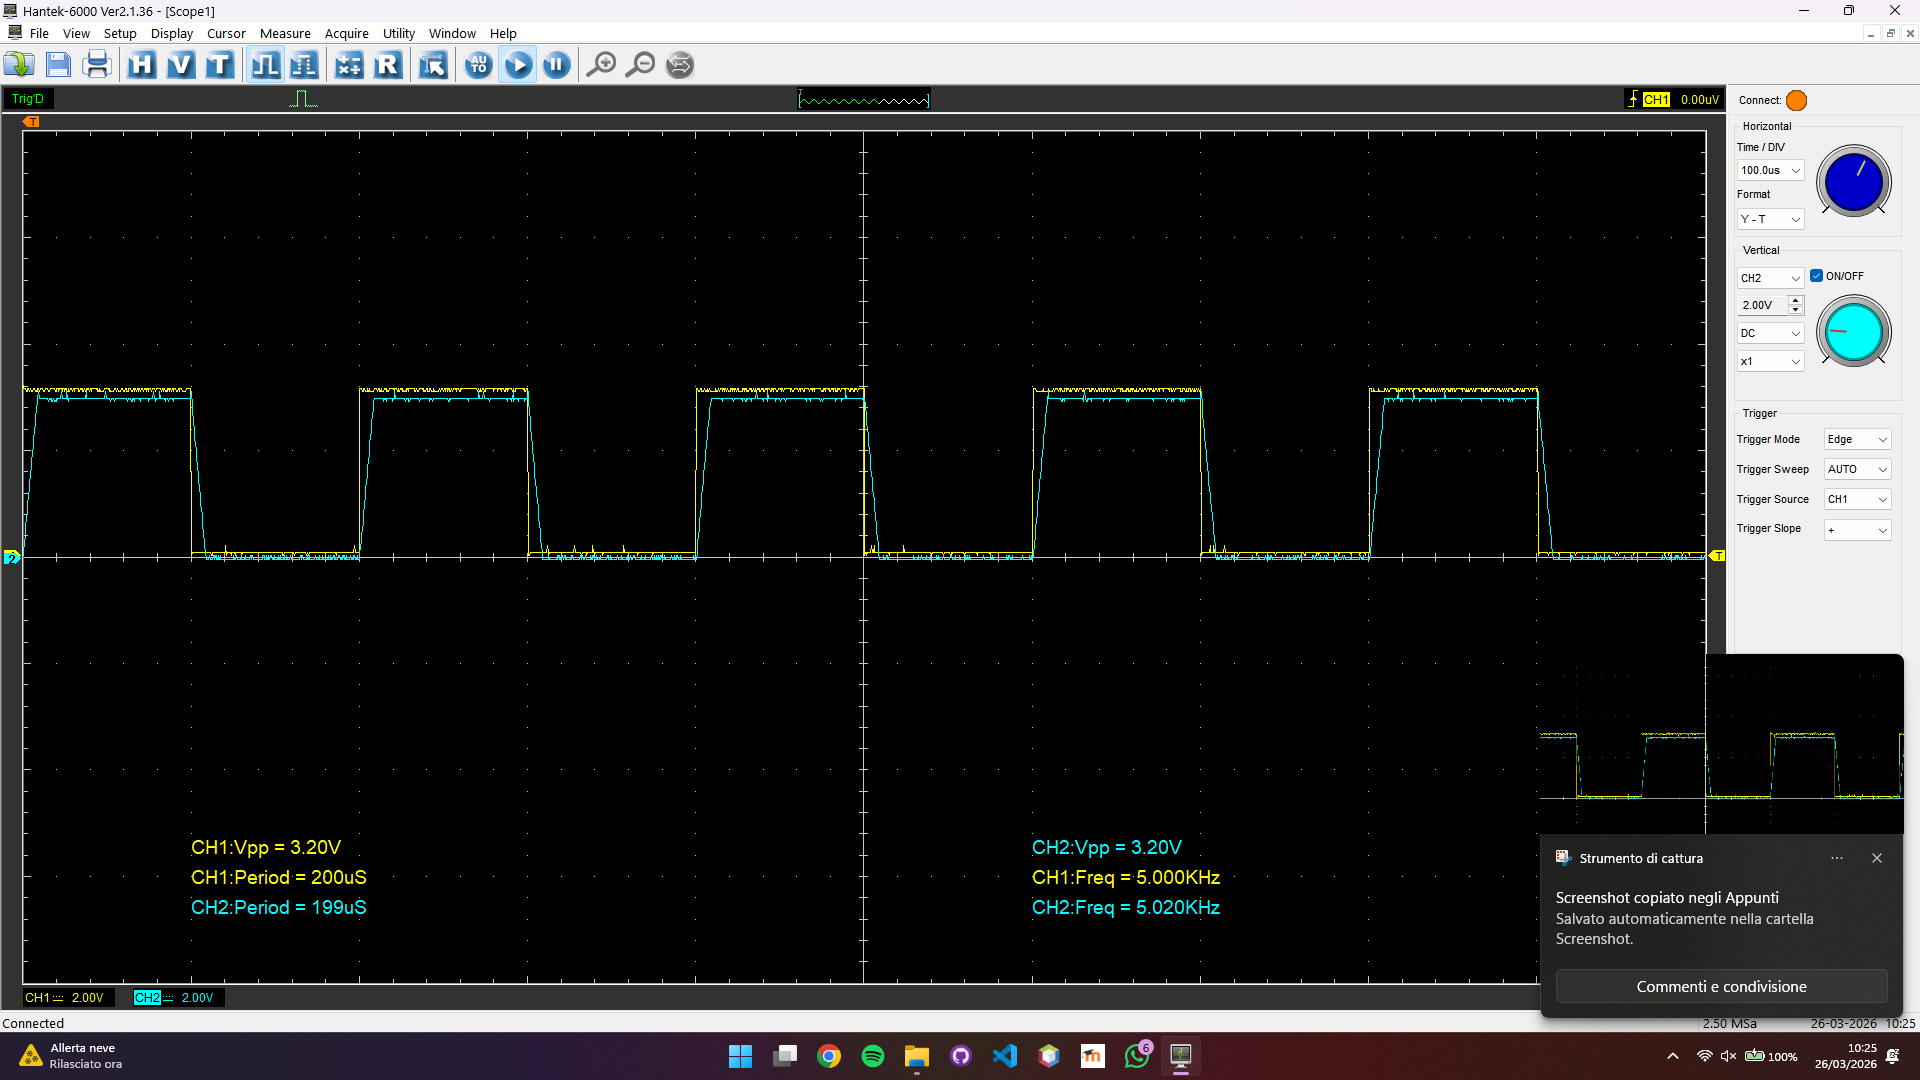
\includegraphics[width=0.7\textwidth]{Misc/Voltage Follower.png}
        \captionsetup{justification=centering, singlelinecheck=false, font=small}
        \caption{Voltage Follower funzionante}
      \end{figure}

      \begin{figure}[H]
        \centering
        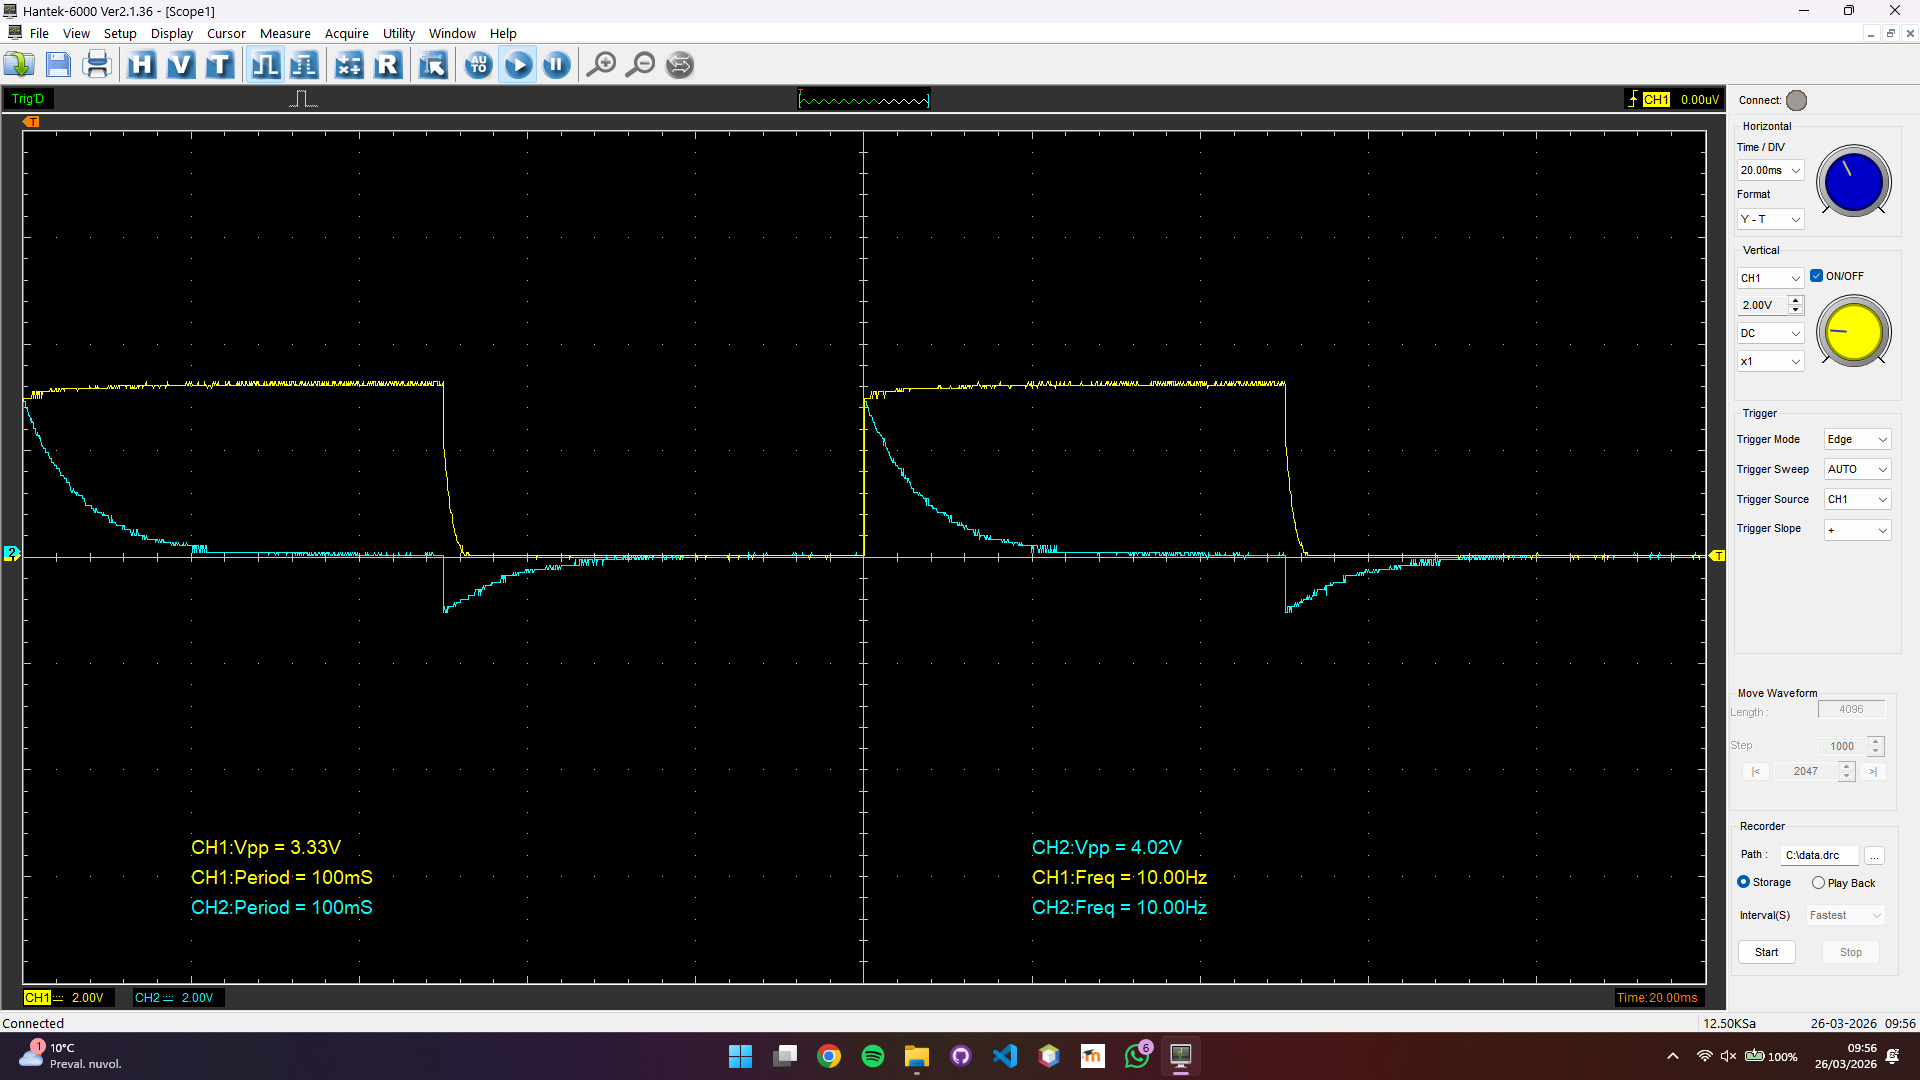
\includegraphics[width=0.7\textwidth]{Misc/10hz BPF.png}
        \captionsetup{justification=centering, singlelinecheck=false, font=small}
        \caption{Onda quadra a 10 Hz}
      \end{figure}

      \begin{figure}[H]
        \centering
        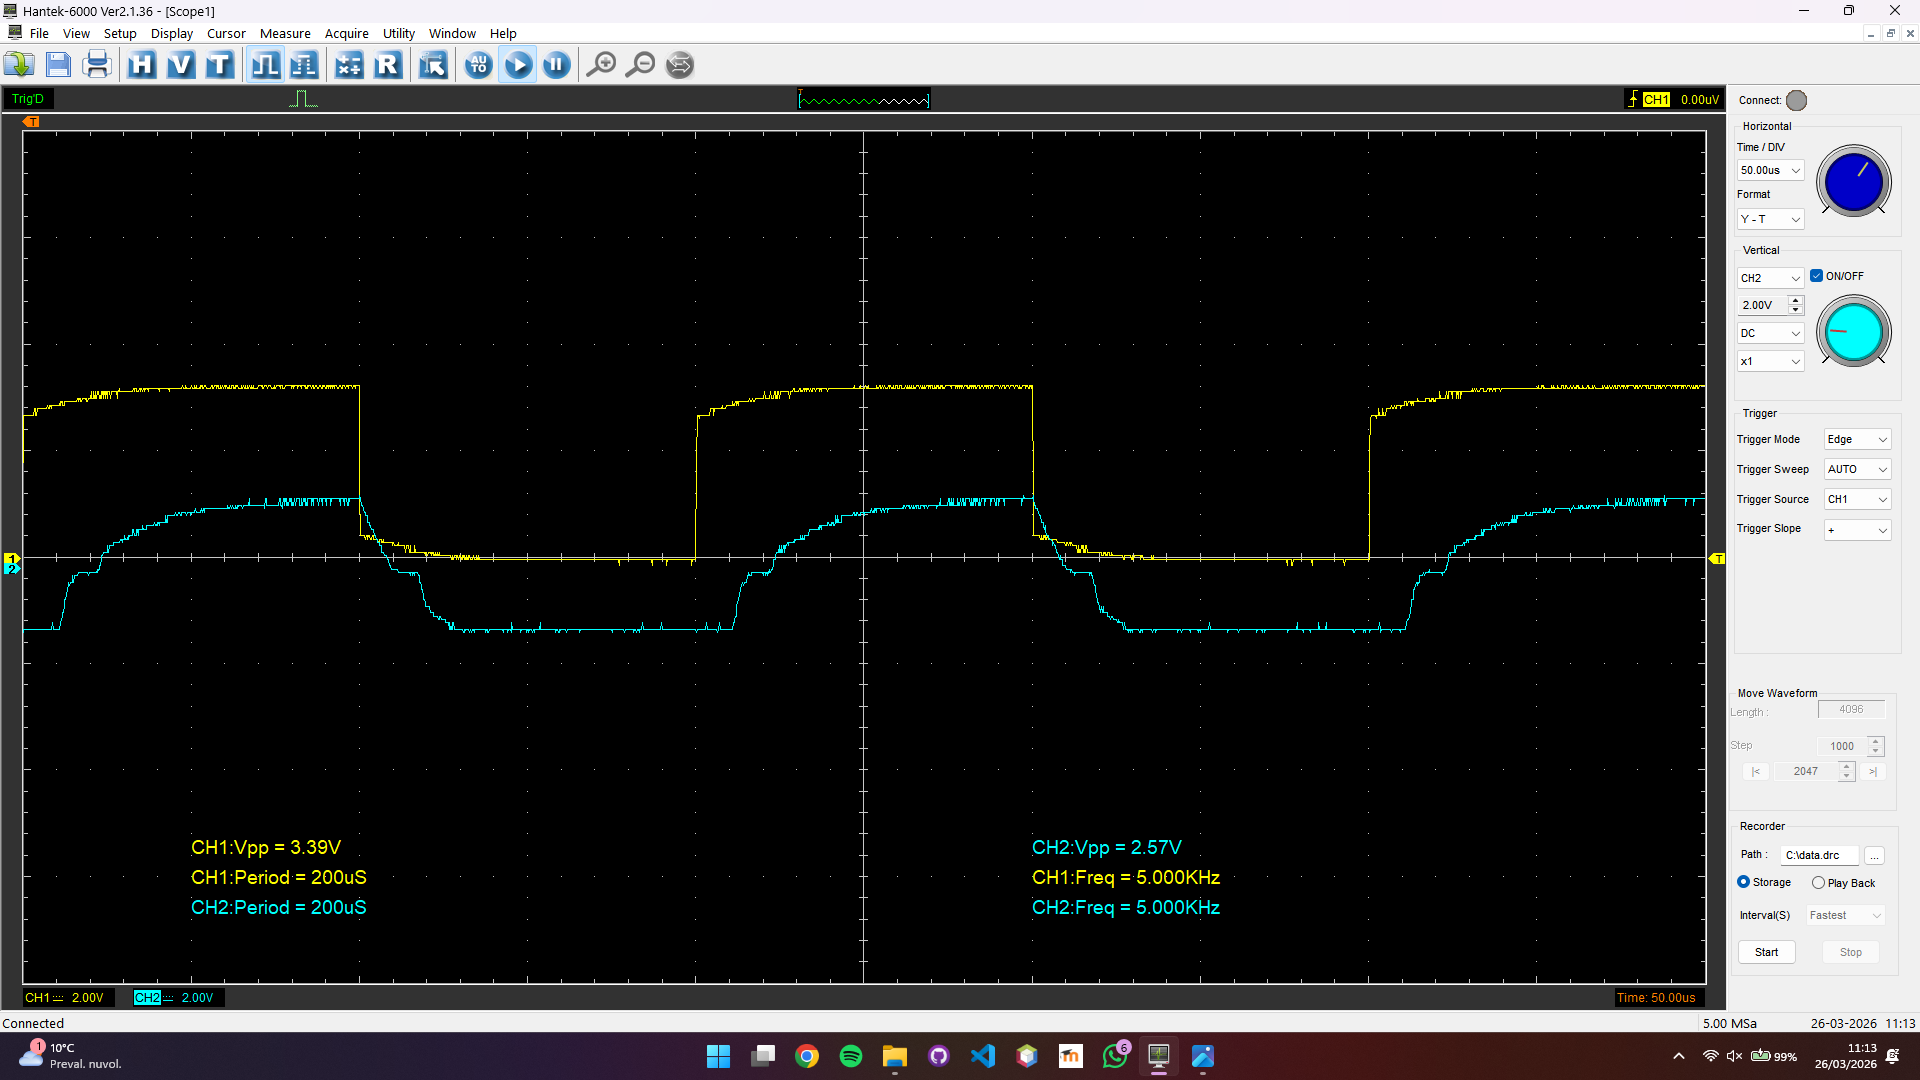
\includegraphics[width=0.7\textwidth]{Misc/5khz BPF.png}
        \captionsetup{justification=centering, singlelinecheck=false, font=small}
        \caption{Onda quadra a 5 kHz}
      \end{figure}

      \begin{figure}[H]
        \centering
        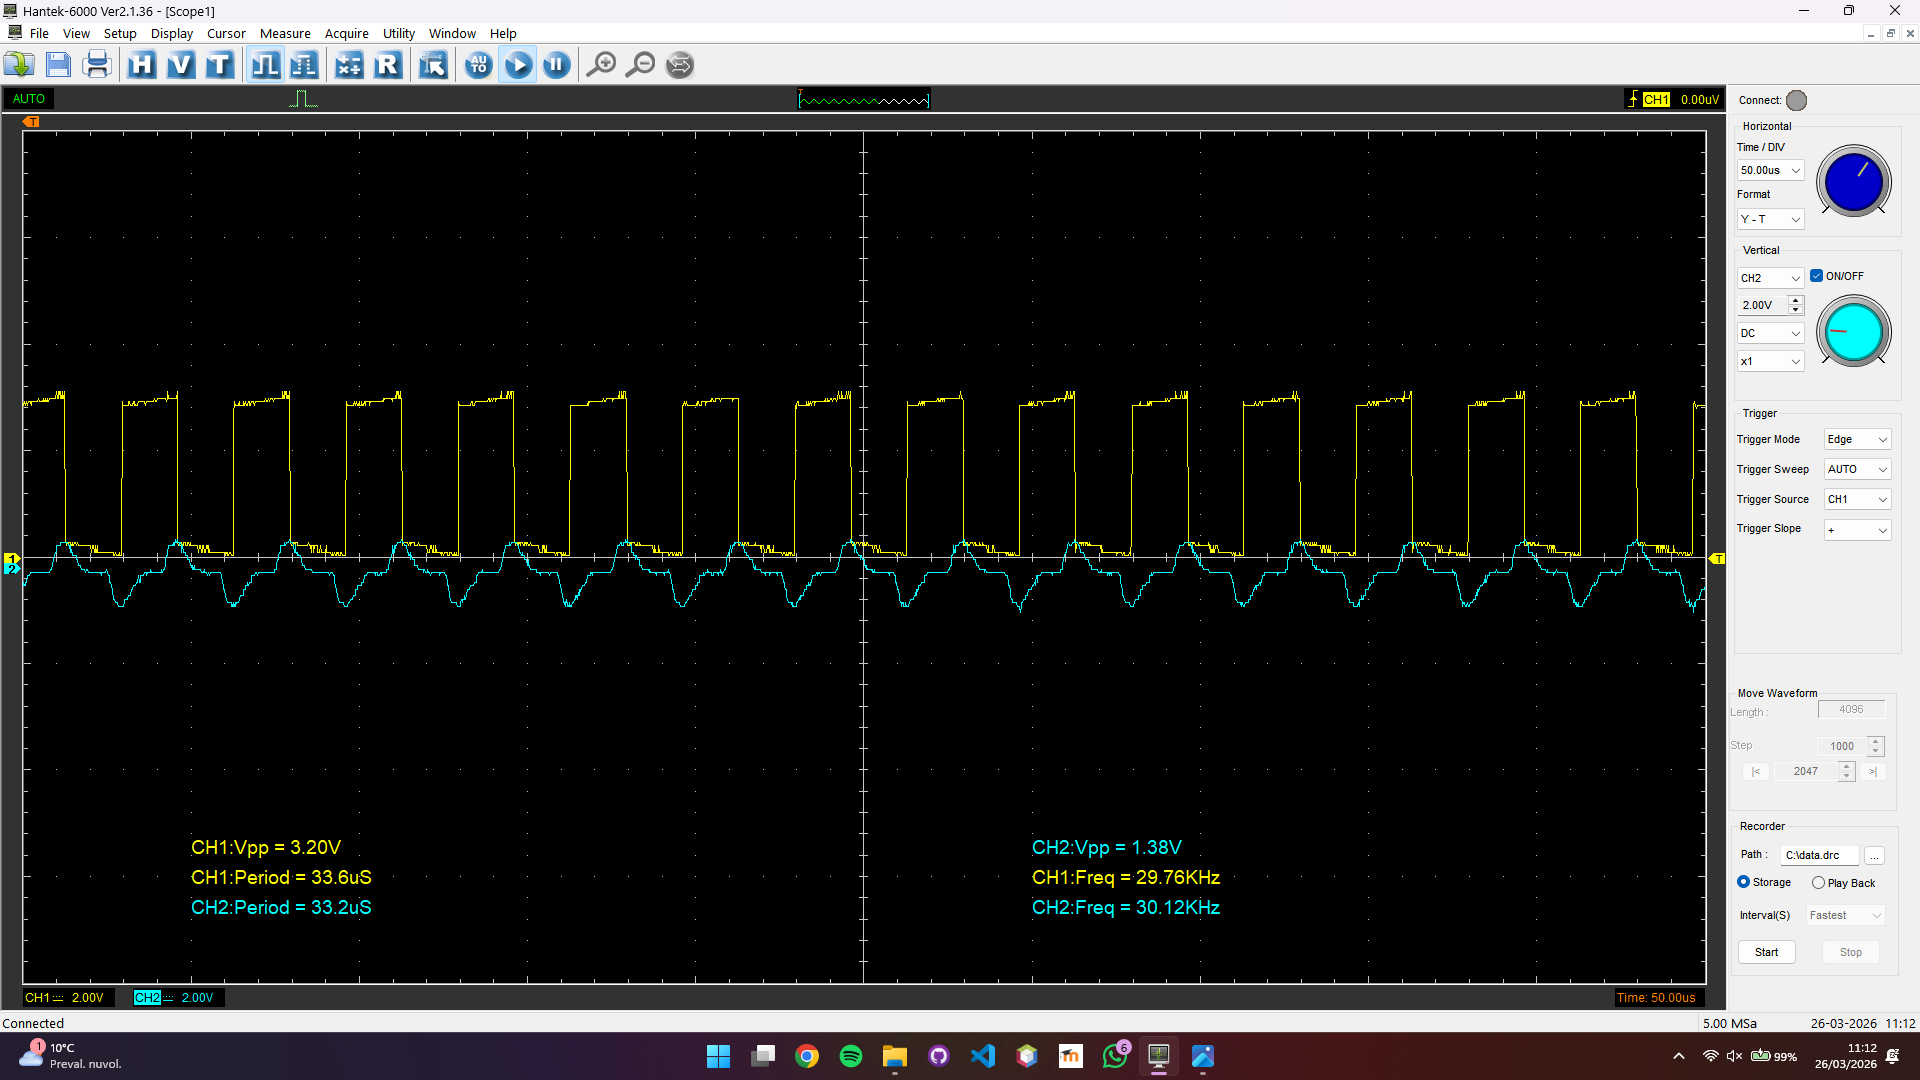
\includegraphics[width=0.7\textwidth]{Misc/30khz BPF.png}
        \captionsetup{justification=centering, singlelinecheck=false, font=small}
        \caption{Onda quadra a 30 kHz}
      \end{figure}

      \item In \textit{Figura 11}, possiamo notare come il comportamento del voltage follower tende proprio
            al comportamento desiderato, ovvero di "inseguire" la tensione applicata agli ingressi invertente e
            non invertente (Ovviamente con le dovute approssimazioni dovute a eventuali comportamenti non ideali
            e ritardi di propagazione verso l'uscita che introduce evitabilmente dei ritardi di fase, seppur minimi).

      \item In \textit{Figura 12}, è illustrato il comportamento del filtro con un ingresso a 10 Hz. A queste frequenze
            agisce solo l'azione del filtro passa-alto ed è particolarmente interessante il comportamento dell'uscita in
            corrispondenza dei fronti di salita e di discesa dell'onda quadra in ingresso. Il condensatore del passa-alto è
            inizialmente scarico. Poiché la tensione ai capi di un condensatore non può variare istantaneamente, l'intero
            sbalzo di tensione si trasferisce immediatamente sull'uscita. Infatti l'onda azzurra schizza verso l'alto nello
            stesso identico istante dell'onda gialla. Subito dopo il salto, la tensione gialla rimane costante. Il condensatore
            comincia a caricarsi attraverso la resistenza del filtro. Man mano che il condensatore si carica, la corrente nel
            circuito diminuisce e la tensione sulla resistenza crolla verso lo zero con l'andamento esponenziale tipico $e^{-t/\tau}$.
            Al momento del fronte di discesa invece succede l'esatto contrario, evidenziando così un comportamento tendente
            ad un circuito derivatore.

      \item In \textit{Figura 13}, osserviamo il comportamento del filtro con un ingresso al centro della banda passante,
            ovvero a 5 kHz. Si può notare come il comportamento tende a quello atteso, l'unica nota da chiarire è il fenomeno
            dello smussamento degli angoli vivi che, come per il caso descritto in precedenza con il filtro passa-basso, si
            manifesta perchè gli angoli vivi sono una caratteristica della componente ad alta frequenza del segnale che viene
            tagliata quasi interamente(in questo caso le armoniche a frequenze superiori sono del tipo (2k-1)5000, $\forall k \in \mathbb{Z}^+$).
            Inoltre la piccola attenuazione che notiamo è perchè 5 kHz è una frequenza che si trova in corrispondenza dell'area
            del diagramma di Bode dove inizia la gamma di alte frequenze da tagliare.

      \item In \textit{Figura 14}, si può osservare il comportamento del filtro con un ingresso a 30 kHz, abbastanza al di sopra
            del limite superiore della banda passante. A $30\text{ kHz}$, il filtro passa-basso si comporta quasi come un integratore,
            infatti tutte le armoniche superiori sono state completamente eliminate; l'unica componente che riesce a transitare, seppur debole,
            è la fondamentale a $30\text{ kHz}$ (che viene integrata da onda quadra a una sorta di onda triangolare/sinusoidale smussata).
            Questo comportamento è anagolo al comportamento del filtro a basse frequenze, solo che qui predomina il lavoro del filtro passa-basso.
    \end{itemize}

  \subsection{Conclusioni}
    L'esperienza ha permesso di verificare sperimentalmente il comportamento di un filtro passa-banda
    RC soggetto a un segnale PWM variabile in frequenza. Il filtro si è dimostrato efficace per lavorare
    con componenti armoniche in varie gamme di frequenze, reagendo come previsto dai calcoli teorici e 
    mostrando tutti gli aspetti tecnici attesi (smussamento angoli vivi, attenuazioni e distorsioni fisiologiche, etc...). 
    Tutte le prove sperimentali hanno quindi evidenziato correttamente tutti gli effetti attesi, in particolare il comportamento
    duale del filtro a bassissime e altissime frequenze presentando un comportamento tendente ad un integratore e ad un derivatore.
    L'accuratezza delle previsioni teoriche è stata in parte limitata da fattori pratici come tolleranze dei componenti, comportamento non ideale
    del segnale PWM, e strumenti di misura, ma resta nel complesso coerente con le aspettative.
\end{document}

